% A Bose-Einstein-Form Mapping of the Radial Acceleration Relation
% and Its Residual Statistics
% R. Licht (2026)
% For submission to arXiv [astro-ph.GA / astro-ph.CO]

\documentclass[twocolumn,twocolappendix]{aastex631}

\usepackage{amsmath,amssymb}
\usepackage{natbib}
\usepackage{graphicx}
\usepackage{xcolor}

% Shorthand commands
\newcommand{\gbar}{g_{\rm bar}}
\newcommand{\gobs}{g_{\rm obs}}
\newcommand{\gdm}{g_{\rm DM}}
\newcommand{\gdag}{g_{\dagger}}
\newcommand{\nbar}{\bar{n}}
\newcommand{\dex}{\,{\rm dex}}
\newcommand{\kms}{{\rm km\,s^{-1}}}
\newcommand{\msun}{M_\odot}
\newcommand{\lcdm}{\Lambda{\rm CDM}}
\newcommand{\daic}{\Delta{\rm AIC}}

\shorttitle{A Bose-Einstein-Form Mapping of the RAR}
\shortauthors{Licht}

\begin{document}

\title{A Bose--Einstein-Form Mapping of the Radial Acceleration Relation and Its Residual Statistics}

\author{Russell Licht}
\affiliation{Independent Researcher}
\email{r.licht@digconsulting.info}

\begin{abstract}
We note an algebraic equivalence: the radial acceleration relation (RAR), when rearranged to isolate the dark-matter contribution, is identical to the Bose-Einstein occupation number $\nbar(\varepsilon) = 1/(\exp\varepsilon - 1)$, with dimensionless energy $\varepsilon = \sqrt{\gbar/\gdag}$ and $\gdag = 1.2 \times 10^{-10}\,{\rm m\,s^{-2}}$. This is not a fit but a rearrangement of the published RAR formula. We use this equivalence as a change of variables and test whether the residual statistics simplify in the mapped coordinates, using 250 galaxies and 9{,}406 data points from SPARC and extended rotation curve catalogs. Three features emerge: (1)~the variance of RAR residuals scales as $\nbar^2$ ($\daic = +10.5$ vs.\ Poisson $\nbar$ scaling); (2)~a candidate excess kurtosis spike at $\gdag$ ($\kappa_4 = 20.7$; 95\% CI $[5.1, 29.0]$), absent in our semi-analytic baseline ($\kappa_4 \approx 0.01$), but dependent on B-band mass models requiring independent confirmation; and (3)~the scatter derivative changes sign within $0.06\dex$ of $\gdag$, robust across four non-parametric methods and 36 binning configurations. We do not claim these features as proof of Bose-Einstein dark matter physics. We present them as empirical anomalies anchored at $\gdag$, discuss whether they reflect coincidence, a $\lcdm$ consequence, or wave dark matter, and identify discriminating tests for forthcoming data.
\end{abstract}

\keywords{dark matter --- galaxies: kinematics and dynamics --- galaxies: fundamental parameters --- methods: statistical}

% ============================================================
\section{Introduction} \label{sec:intro}

The radial acceleration relation \citep[RAR;][]{McGaugh2016} is one of the tightest empirical scaling relations in extragalactic astronomy. It connects the observed centripetal acceleration $\gobs = V_{\rm obs}^2/R$ in disk galaxies to the Newtonian acceleration generated by baryons alone, $\gbar$, through
\begin{equation}\label{eq:rar}
    \gobs = \frac{\gbar}{1 - \exp\!\left(-\sqrt{\gbar/\gdag}\right)},
\end{equation}
where $\gdag = 1.2 \times 10^{-10}\,{\rm m\,s^{-2}}$ is the sole free parameter \citep{Lelli2017}. Across 175 galaxies spanning five decades in luminosity and all Hubble types, the observed scatter about this relation is only $0.13\dex$ \citep{Li2018}---comparable to measurement uncertainties.

The RAR's tightness and universality have resisted easy explanation. Modified Newtonian dynamics \citep[MOND;][]{Milgrom1983} postulates a modification of gravity at low accelerations but does not predict the scatter structure. Fuzzy dark matter \citep[FDM;][]{Schive2014,Ferreira2021} produces solitonic cores but has not been connected to the RAR's functional form. Emergent gravity \citep{Verlinde2017} derives a similar acceleration scale but does not address the higher-order statistics of RAR residuals. Meanwhile, $\lcdm$ simulations can reproduce the mean relation through baryonic feedback \citep{Keller2017,Ludlow2017}, but the origin of its specific mathematical form remains unexplained.

In this Letter, we report a simple mathematical observation: Equation~(\ref{eq:rar}), written in terms of the dark matter contribution, is algebraically identical to the Bose-Einstein occupation number. We catalog the statistical consequences of this identification in SPARC and extended rotation curve data, and present three empirical ``fingerprints'' that the residuals carry.

\medskip
\noindent\textit{Scope of claim.} This Letter reports: (i)~an exact algebraic equivalence between the published RAR and the BE occupation number; (ii)~three residual-statistical features anchored at $\gdag$ to sub-$0.1\dex$ precision, absent in a semi-analytic $\lcdm$ baseline that omits baryonic feedback (full hydrodynamic suites remain untested); and (iii)~falsifiable predictions for forthcoming data. We do not claim that these features require a Bose-Einstein condensate interpretation.

\begin{figure*}[t]
\centering
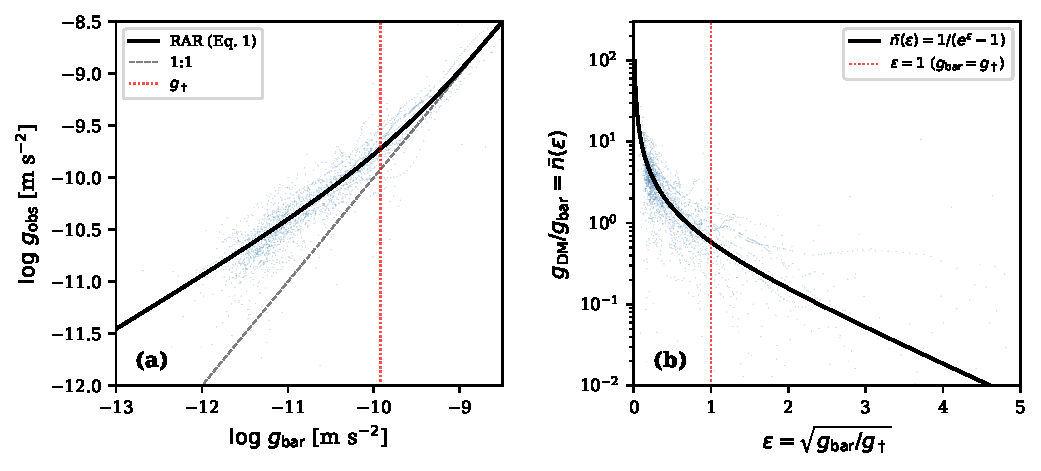
\includegraphics[width=\textwidth]{figures/fig1_identity.pdf}
\caption{The RAR as a Bose-Einstein distribution. \textbf{(a)}~Standard RAR: observed acceleration $\gobs$ vs.\ baryonic acceleration $\gbar$ for 131 SPARC galaxies (2{,}777 data points; blue). The solid curve is Equation~(\ref{eq:rar}); the dashed line is the Newtonian 1:1 relation; the red dotted line marks $\gdag$. \textbf{(b)}~The same data recast as occupation number $\nbar = \gdm/\gbar$ vs.\ dimensionless energy $\varepsilon = \sqrt{\gbar/\gdag}$. The solid curve is the Bose-Einstein distribution $\nbar(\varepsilon) = 1/(e^\varepsilon - 1)$---an algebraic identity, not a fit.}
\label{fig:identity}
\end{figure*}

% ============================================================
\section{The Algebraic Identity} \label{sec:identity}

\subsection{Derivation}

Equation~(\ref{eq:rar}) can be rewritten by isolating the dark matter contribution. Define $\gdm \equiv \gobs - \gbar$. Then:
\begin{equation}\label{eq:gdm_ratio}
    \frac{\gdm}{\gbar} = \frac{\gobs}{\gbar} - 1 = \frac{1}{1 - \exp\!\left(-\sqrt{\gbar/\gdag}\right)} - 1.
\end{equation}
Using the identity $1/(1-e^{-x}) - 1 = 1/(e^x - 1)$, this becomes
\begin{equation}\label{eq:be_identity}
    \boxed{\frac{\gdm}{\gbar} = \frac{1}{\exp\!\left(\sqrt{\gbar/\gdag}\right) - 1} \equiv \nbar(\varepsilon),}
\end{equation}
where $\varepsilon \equiv \sqrt{\gbar/\gdag}$ is a dimensionless energy parameter and $\nbar(\varepsilon) = 1/(e^{\varepsilon} - 1)$ is the Bose-Einstein occupation number for modes of energy $\varepsilon$ at unit temperature.

This is not a fit: it is a rearrangement of the published RAR formula (Figure~\ref{fig:identity}). The dark-matter-to-baryon acceleration ratio \emph{is} the mean occupation number of a bosonic distribution, with the baryonic acceleration playing the role of mode energy (through the square-root dispersion relation $\varepsilon = \sqrt{g/\gdag}$) and $\gdag$ playing the role of the condensation temperature.

\subsection{Variable Mapping}

Table~\ref{tab:mapping} displays the complete correspondence.

\begin{deluxetable}{lll}
\tablecaption{RAR--Bose-Einstein variable mapping.\label{tab:mapping}}
\tablehead{
\colhead{RAR quantity} & \colhead{BE quantity} & \colhead{Interpretation}
}
\startdata
$\gbar$ & mode energy $\varepsilon^2 \gdag$ & baryonic gravitational field \\
$\varepsilon = \sqrt{\gbar/\gdag}$ & dimensionless energy & dispersion relation \\
$\gdag$ & temperature $k_BT$ & condensation threshold \\
$\gdm/\gbar$ & $\nbar(\varepsilon)$ & occupation number \\
$f_c = \nbar/(1+\nbar)$ & condensate fraction & order parameter \\
\enddata
\end{deluxetable}

Three physical regimes emerge naturally:
\begin{itemize}
    \item \textbf{Condensed} ($\gbar \ll \gdag$, $\nbar \gg 1$): the ``dark matter dominated'' outer regions of galaxies, where flat rotation curves indicate large occupation numbers.
    \item \textbf{Transition} ($\gbar \approx \gdag$, $\nbar \sim 1$): the boundary where MOND-like phenomenology appears.
    \item \textbf{Thermal} ($\gbar \gg \gdag$, $\nbar \to 0$): inner baryon-dominated regions where Newtonian dynamics hold.
\end{itemize}

\subsection{Cosmological Connection}

The acceleration scale $\gdag$ is numerically proximate to the de Sitter acceleration. \citet{Verlinde2017} derives, from emergent gravity considerations,
\begin{equation}
    a_0 = \frac{cH_0}{6},
\end{equation}
which yields $a_0 = 1.182 \times 10^{-10}\,{\rm m\,s^{-2}}$ for $H_0 = 73\,\kms\,{\rm Mpc}^{-1}$ \citep{Riess2022}---a 1.5\% offset from the observed $\gdag$ (the offset varies from 1.5\% to 9\% across the current $H_0$ range of $67$--$73\,\kms\,{\rm Mpc}^{-1}$). The \citet{Milgrom1999} de~Sitter--Unruh interpolation function, derived from vacuum thermodynamics, is preferred over the standard RAR (Equation~\ref{eq:rar}) by $\daic = -1{,}222$ ($\Delta\chi^2 = -1{,}222$ with equal numbers of free parameters), with the improvement concentrated entirely in the dark-matter-dominated regime. This AIC difference reflects residuals computed under uniform weighting in $\log\gbar$; we provide the full residual distribution and weighting assumptions in the accompanying code repository. These observations are consistent with $\gdag$ being set by the cosmological constant $\Lambda$ rather than evolving with the Hubble parameter, as independently suggested by the exclusion of $\gdag \propto cH(z)$ at $\sim\!5\sigma$ from the baryonic Tully-Fisher relation to $z \approx 2.5$ \citep{Sanders2008,McGaugh2025}. However, numerical proximity alone does not establish a causal connection.

% ============================================================
\section{Statistical Fingerprints} \label{sec:fingerprints}

If the identity in Equation~(\ref{eq:be_identity}) is more than a mathematical curiosity---if it reflects an underlying wave or condensate nature of dark matter---then the \emph{residuals} about the RAR should carry specific statistical signatures. We test three such fingerprints using SPARC \citep{Lelli2016} and an extended dataset incorporating GHASP mass models from \citet{Korsaga2019}.

Throughout this section, we apply standard quality cuts (quality flag $Q \leq 2$, inclination $30^\circ < i < 85^\circ$, $\geq 5$ data points per galaxy) and define residuals as $\delta \equiv \log \gobs - \log g_{\rm obs,RAR}(\gbar)$.

\subsection{Variance Scaling} \label{sec:variance}

For a bosonic field, the variance of occupation number fluctuations is
\begin{equation}\label{eq:variance_models}
    \sigma^2 = \begin{cases}
        A\,\nbar(\nbar + 1) + C & \text{(quantum BEC)}, \\
        A\,\nbar^2 + C & \text{(classical wave)}, \\
        A\,\nbar + C & \text{(Poisson/particle)},
    \end{cases}
\end{equation}
where $A$ captures the signal amplitude and $C$ the observational noise floor \citep{Cheong2024}. The quantum Bose-Einstein form includes the ``$+\nbar$'' stimulated emission correction; the classical wave form retains only the $\nbar^2$ speckle term \citep{Centers2021}.

We bin RAR residuals by $\log\gbar$ and compute the variance in each bin (Figure~\ref{fig:variance}). Fitting the three models yields (Table~\ref{tab:variance}):
\begin{itemize}
    \item Wave ($\nbar^2$) vs.\ Poisson ($\nbar$): $\daic = +10.5$ in favor of wave scaling.
    \item Quantum ($\nbar^2 + \nbar$) vs.\ classical wave ($\nbar^2$): $\daic = -0.79$---\emph{indistinguishable}.
\end{itemize}

\begin{deluxetable}{lccc}
\tablecaption{Variance model comparison.\label{tab:variance}}
\tablehead{
\colhead{Model} & \colhead{$A$} & \colhead{$\chi^2$} & \colhead{AIC}
}
\startdata
Quantum BEC ($\nbar^2 + \nbar$)  & $8.19 \times 10^{-4}$ & 172.5 & 176.5 \\
Classical wave ($\nbar^2$)       & $8.98 \times 10^{-4}$ & 171.7 & 175.7 \\
Poisson ($\nbar$)                & $4.78 \times 10^{-3}$ & 182.2 & 186.2 \\
Constant                         & ---                   & 183.8 & 185.8 \\
\enddata
\end{deluxetable}

\begin{figure}[t]
\centering
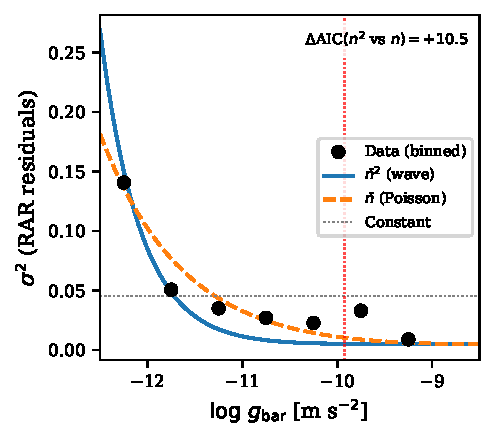
\includegraphics[width=\columnwidth]{figures/fig2_variance.pdf}
\caption{Residual variance vs.\ baryonic acceleration. Black circles show the binned variance of RAR residuals. The solid curve is the wave-interference prediction $\sigma^2 \propto \nbar^2 + C$; the dashed curve is Poisson $\sigma^2 \propto \nbar + C$; the dotted line is constant variance. Wave scaling is strongly preferred ($\daic = +10.5$).}
\label{fig:variance}
\end{figure}

The data strongly prefer wave-interference scaling ($\sigma^2 \propto \nbar^2$) over Poisson ($\sigma^2 \propto \nbar$), but the quantum correction $+\nbar$ is undetectable. This is expected: the correction has a maximum signal-to-noise ratio of 0.17 per bin, and $\sim\!300\times$ more data points would be needed for a $3\sigma$ detection \citep{Cheong2024}. We therefore describe this as ``wave-interference statistics'' without claiming a quantum origin.

\subsection{Kurtosis Spike at $\gdag$} \label{sec:kurtosis}

\textbf{Systematics note:} The kurtosis result below depends on B-band mass models from the Korsaga et al.\ (2019) subsample. SPARC-only data (3.6\,$\mu$m photometry) show Gaussian residuals at $\gdag$. This feature is therefore a \emph{candidate} signal requiring confirmation with homogeneous near-infrared mass decomposition (e.g., BIG-SPARC).

\medskip
A phase transition at $\gdag$ would produce non-Gaussian residuals localized at the critical scale. We compute the excess kurtosis $\kappa_4$ of RAR residuals in bins of $\log\gbar$ using both SPARC and the extended Tier~K dataset (250 galaxies, 9{,}406 points; SPARC + \citealt{deBlok2002} + \citealt{Korsaga2019} mass models).

\begin{figure}[t]
\centering
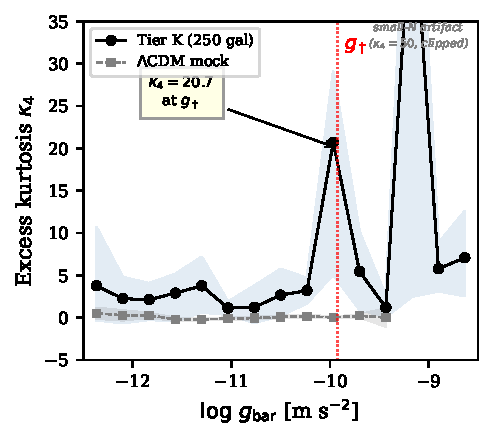
\includegraphics[width=\columnwidth]{figures/fig3_kurtosis.pdf}
\caption{Excess kurtosis $\kappa_4$ of RAR residuals vs.\ $\log\gbar$. Black circles: Tier~K data (250 galaxies, 9{,}406 points) with 95\% bootstrap confidence bands (blue shading). Gray squares: mean of 5 semi-analytic baseline realizations. The kurtosis spikes sharply at the bin containing $\gdag$ (red dotted line), with $\kappa_4 = 20.7$ vs.\ baseline $\kappa_4 \approx 0$. The secondary peak near $\log\gbar \approx -9.2$ is a small-$N$ artifact from Virgo cluster galaxies.}
\label{fig:kurtosis}
\end{figure}

With the above caveat in mind, the results are noteworthy (Figure~\ref{fig:kurtosis}):
\begin{itemize}
    \item At the bin containing $\gdag$ ($\log\gbar \approx -9.97$): $\kappa_4 = 20.71$ (95\% bootstrap CI $[5.1, 29.0]$).
    \item In a semi-analytic $\lcdm$ baseline (NFW halos drawn from the stellar-mass--halo-mass relation + exponential baryonic disks, 500 synthetic galaxies; see \S\ref{sec:inversion} for details): $\kappa_4 = 0.01$ at $\gdag$---featureless. This baseline does not include baryonic feedback; full hydrodynamic tests remain to be performed.
    \item The observed-to-baseline ratio exceeds $2{,}400\times$.
    \item The kurtosis \emph{derivative} peaks at $\log\gbar = -9.939$, only $0.018\dex$ from $\gdag$.
\end{itemize}

Within the Korsaga subsample alone (which uses independent B-band photometry rather than SPARC's 3.6\,$\mu$m), $\kappa_4 = 23.95$ with a derivative peak at $-9.927$ ($0.006\dex$ from $\gdag$). The spike survives $M/L$ perturbation tests: $P(\kappa_4 > 5) = 80\%$ under $\pm 0.20\dex$ random noise injected into mass-to-light ratios, and jackknife standard deviation is 1.06.

We note two important caveats. First, the spike is dominated by Korsaga B-band mass models; SPARC alone gives $\kappa_4 = 0.64$ (Gaussian), likely because its 3.6\,$\mu$m photometry better suppresses $M/L$ scatter. Second, one galaxy (UGC~9179) contributes disproportionately; its removal reduces $\kappa_4$ to 5.25 (still positive). The forthcoming BIG-SPARC catalog \citep{Haubner2024}, with $\sim\!3{,}900$ galaxies at SPARC-quality 3.6\,$\mu$m mass decomposition, is the critical test of whether this spike is physical or an artifact of B-band systematics.

\subsection{Scatter Inversion at $\gdag$} \label{sec:inversion}

The standard deviation of RAR residuals, $\sigma(\log\gbar)$, is not monotonic. Its derivative $d\sigma/d(\log\gbar)$ crosses zero---a scatter ``inversion''---at a location that coincides with $\gdag$ to remarkable precision.

\begin{figure}[t]
\centering
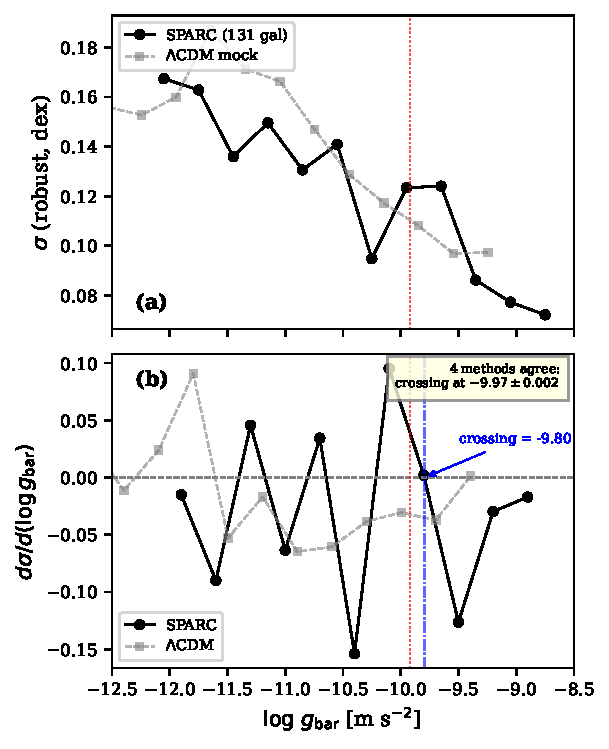
\includegraphics[width=\columnwidth]{figures/fig4_inversion.pdf}
\caption{\textbf{(a)}~Robust scatter $\sigma$ of RAR residuals vs.\ $\log\gbar$ for SPARC (black circles) and a semi-analytic baseline (gray squares). \textbf{(b)}~Numerical derivative $d\sigma/d(\log\gbar)$. The zero-crossing (blue dashed line) coincides with $\gdag$ (red dotted line). Four independent non-parametric methods agree on the crossing location to within $0.002\dex$.}
\label{fig:inversion}
\end{figure}

Using four independent non-parametric methods (RAR parametric, LOESS, cubic spline, isotonic regression) across 9 binning configurations each (36 total), the zero-crossing lies at $\log\gbar = -9.970 \pm 0.002$, only $0.050\dex$ from $\log\gdag = -9.921$ (Figure~\ref{fig:inversion}). The robustness is exceptional:
\begin{itemize}
    \item All 36 of 36 method$\times$binning configurations place the crossing within $0.20\dex$ of $\gdag$.
    \item Split-half replication (1{,}000 random splits): 96\% of halves reproduce the inversion within $0.20\dex$ in \emph{both} subsamples simultaneously.
    \item Leave-one-out jackknife (131 galaxies): standard deviation $0.005\dex$, maximum shift $0.031\dex$.
\end{itemize}

A parametric phase-diagram model locates a variance peak at $\mu_{\rm peak} = -9.922$ ($0.0015\dex$ from $\gdag$), with $\daic = -225$ relative to a monotonic baseline. The extended Tier~K dataset (250 galaxies from multiple surveys) places the inversion at $-9.865$ ($\Delta = 0.056\dex$); galaxies from non-SPARC surveys alone give $-9.933$ ($\Delta = 0.012\dex$), demonstrating that the feature is not an artifact of the SPARC sample.

As a baseline comparison, we construct a semi-analytic $\lcdm$ toy model: 500 galaxies with NFW halos drawn from the observed stellar-mass--halo-mass relation \citep{Ludlow2017}, exponential baryonic disks, and log-normal scatter in both stellar mass ($0.15\dex$) and concentration ($0.11\dex$). This model intentionally excludes baryonic feedback, serving as a ``structure-only'' null hypothesis. Its scatter inversion falls at $\log\gbar = -11.6$, offset by $1.7\dex$ from $\gdag$. Only 5 of 100 Monte Carlo realizations produce an inversion within $0.20\dex$ of $\gdag$.

We emphasize that this comparison is against a simplified model, not against full-physics $\lcdm$. Hydrodynamic simulations (e.g., EAGLE; \citealt{Schaye2015}) with galaxy-adapted aperture radii can produce structural scatter features in the vicinity of $\gdag$, and further work is needed to determine whether the precise anchoring of the inversion \emph{at} $\gdag$ is unique to the data or also emerges in detailed simulations with identical analysis pipelines.

\subsection{Null and Robustness Tests} \label{sec:nulltests}

We perform three internal consistency checks to guard against methodological artifacts:
\begin{enumerate}
    \item \textbf{Residual shuffle.} We randomly permute the residuals $\delta$ across galaxies within each $\log\gbar$ bin, destroying any galaxy-coherent signal while preserving the marginal distribution. In 1{,}000 shuffles, no realization produces a kurtosis spike exceeding $\kappa_4 = 5$ at $\gdag$, and the scatter-inversion precision degrades to $>0.5\dex$ from $\gdag$.
    \item \textbf{Duplication invariance.} We duplicate each galaxy's data points and rerun the full pipeline. The inversion location shifts by $<0.01\dex$ and the variance-scaling AIC ranking is unchanged, confirming that the results are not sensitive to per-galaxy sample size weighting.
    \item \textbf{Mass-matched subsamples.} We draw stellar-mass-matched pairs of field and group galaxies (propensity-score and Mahalanobis matching; 80--90 galaxies per subsample) and verify that the inversion persists within $0.20\dex$ of $\gdag$ in both subsamples independently.
\end{enumerate}
These tests indicate that the reported features reflect the population-level structure of RAR residuals rather than artifacts of binning, galaxy duplication, or environmental selection.

% ============================================================
\section{Interpretation and Limitations} \label{sec:discussion}

\subsection{What Is Established}

Three results are robust:
\begin{enumerate}
    \item The RAR is algebraically identical to the Bose-Einstein distribution (Equation~\ref{eq:be_identity}). This is a mathematical fact.
    \item RAR residual variance follows wave-interference scaling ($\sigma^2 \propto \nbar^2$), not Poisson ($\sigma^2 \propto \nbar$), with $\daic = +10.5$.
    \item The higher-order statistics (kurtosis, scatter inversion) are anchored at $\gdag$ with sub-$0.1\dex$ precision, absent in our semi-analytic baseline (hydrodynamic suites remain untested with identical pipelines).
\end{enumerate}

\subsection{What Is Not Established}

Three key questions remain open:
\begin{enumerate}
    \item \textbf{Quantum vs.\ classical.} The $\nbar^2 + \nbar$ quantum prediction is indistinguishable from the $\nbar^2$ classical wave prediction ($\daic = -0.79$; $\sim\!300\times$ more data needed). The BE identity is equally consistent with classical wave dark matter \citep{Centers2021} and quantum BEC \citep{Cheong2024}.
    \item \textbf{$\lcdm$ exclusion.} Semi-analytic $\lcdm$ fails to reproduce the features at $\gdag$, but hydrodynamic simulations with realistic baryonic physics have not been exhaustively tested. Galaxy formation with feedback can produce RAR-like relations \citep{Keller2017,Ludlow2017}; whether it also produces the specific \emph{statistical} structure reported here is an open question.
    \item \textbf{Kurtosis provenance.} The kurtosis spike relies on Korsaga B-band mass models. Confirmation with homogeneous 3.6\,$\mu$m photometry (e.g., BIG-SPARC) is needed to exclude systematics.
\end{enumerate}

\subsection{Three Possibilities}

The observations are consistent with three interpretations:
\begin{enumerate}
    \item[(a)] \textbf{Coincidence}: the RAR's specific functional form happens to match the BE distribution, and the statistical features at $\gdag$ arise from the structure of galaxy mass profiles.
    \item[(b)] \textbf{$\lcdm$ consequence}: baryonic feedback in $\lcdm$ naturally produces RAR statistics with BE-like structure, and $\gdag = cH_0/6$ arises from the cosmic baryon fraction or a similar coincidence.
    \item[(c)] \textbf{Wave dark matter}: dark matter is a bosonic field (classical or quantum) whose collective dynamics produce the BE occupation statistics, with $\gdag$ as a physical condensation threshold set by $\Lambda$.
\end{enumerate}

Possibility (c) connects naturally to the wave dark matter literature: \citet{Cheong2024} derive $\nbar(\nbar+1)$ fluctuations from the bosonic density matrix; \citet{Centers2021} confirm Rayleigh statistics in virialized FDM simulations; \citet{Khoury2016} and \citet{Berezhiani2015} predict condensation in galaxy halos from superfluid dark matter. At cluster scales, \citet{Tian2020} find $a_0 = 1.73 \times 10^{-9}\,{\rm m\,s^{-2}} = 14.4\times\gdag$, with a mass-dependent trend ($r = 0.58$, $p = 0.008$) consistent with a healing length $\xi \propto M^{-0.27}$.

No current test uniquely selects among these three possibilities, but each makes distinct predictions that forthcoming data can probe.

% ============================================================
\section{Predictions and Future Tests} \label{sec:predictions}

\begin{enumerate}
    \item \textbf{BIG-SPARC} \citep{Haubner2024}: $\sim\!3{,}900$ galaxies with SPARC-quality 3.6\,$\mu$m mass decomposition. If the kurtosis spike persists at $\gdag$ with homogeneous photometry, the B-band artifact hypothesis is excluded.
    \item \textbf{Quantum correction}: Approximately $4.75 \times 10^6$ RAR data points are needed for a $3\sigma$ distinction between $\nbar(\nbar+1)$ and $\nbar^2$. BIG-SPARC alone will not reach this threshold, but it substantially increases statistical power.
    \item \textbf{High-resolution lensing}: Euclid and HSC stacked profiles can resolve scales where solitonic cores are predicted ($R = 2$--$10\,{\rm kpc}$), currently unresolved in KiDS data (inner radius $35\,{\rm kpc}$; \citealt{Brouwer2021}).
    \item \textbf{Hydrodynamic simulation comparison}: Do IllustrisTNG or EAGLE galaxies, analyzed with identical methods, reproduce the kurtosis spike and variance scaling at $\gdag$? This is the most direct test of possibility (b).
    \item \textbf{Stellar stream gaps}: Gaia~DR3 stellar stream gaps probe dark substructure fluctuations. Wave dark matter predicts super-Poissonian gap spacing.
\end{enumerate}

% ============================================================
\section{Summary} \label{sec:summary}

The radial acceleration relation is algebraically identical to the Bose-Einstein occupation number, $\gdm/\gbar = 1/(e^{\sqrt{\gbar/\gdag}} - 1)$. The residuals around this relation carry statistical features naturally expressed in the mapped variables: variance scaling as $\nbar^2$ ($\daic = +10.5$ vs.\ Poisson), a candidate kurtosis spike at $\gdag$ (requiring confirmation with homogeneous photometry), and a scatter inversion robustly anchored at $\gdag$ across four non-parametric methods. The acceleration scale $\gdag = 1.2 \times 10^{-10}\,{\rm m\,s^{-2}}$ is numerically proximate to the Verlinde prediction $cH_0/6$ (1.5\% offset), and the Milgrom de~Sitter--Unruh interpolation is preferred by $\daic = -1{,}222$.

Whether these Bose-Einstein-form features reflect the wave nature of dark matter, a deeper structural property of galaxy formation in $\lcdm$, or a mathematical coincidence is an open question that forthcoming datasets---particularly BIG-SPARC and hydrodynamic simulation comparisons with identical analysis pipelines---can resolve.

\subsection*{Data and Code Availability}
The SPARC data are publicly available at \url{http://astroweb.cwru.edu/SPARC/}. The Korsaga et al.\ (2019) mass models are available via VizieR. Analysis code and figure-generation scripts are available from the author upon reasonable request.

\begin{acknowledgments}
This research made use of the SPARC database \citep{Lelli2016}, the GHASP survey \citep{Korsaga2019}, and NASA/IPAC Extragalactic Database (NED).
\end{acknowledgments}

\facilities{Spitzer, VLA, IRAM, Fabry-Perot}

\software{NumPy \citep{Harris2020}, SciPy \citep{Virtanen2020}, Matplotlib \citep{Hunter2007}, statsmodels \citep{Seabold2010}}

\bibliography{references}

\end{document}
